\documentclass[dvipdfmx, titlepage]{jsarticle}

% \usepackage{geometry}
\usepackage[dvipdfmx]{graphicx}
\usepackage{ascmac}
\usepackage{amsmath}
\usepackage{amssymb}
\usepackage{minted}
\usepackage{listings}
% \usepackage[utf8]{inputenc}
% \usepackage{listingsutf8}
\usepackage{newfloat} % newfloat パッケージを読み込む
\usepackage{caption}
\usepackage{float}
\usepackage{fix-cm}
\usepackage{svg}
\usepackage{enumitem}

\usepackage{hyperref}
% for hyperref
\usepackage{pxjahyper}
\hypersetup{
    dvipdfmx,
	colorlinks=false, % リンクに色をつけない設定
	bookmarks=true, % 以下ブックマークに関する設定
	bookmarksnumbered=true,
	pdfborder={0 0 0},
	bookmarkstype=toc
}

% \lstset{
%   basicstyle={\ttfamily},
%   identifierstyle={\small},
%   inputencoding=auto,
%   commentstyle={\small\sffamily},
%   keywordstyle={\small\bfseries},
%   ndkeywordstyle={\small},
%   stringstyle={\small\ttfamily},
%   frame={tb},
%   breaklines=true,
%   columns=[l]{fullflexible},
%   numbers=left,
%   % xrightmargin=0zw,
%   % xleftmargin=3zw,
%   numberstyle={\scriptsize},
%   firstnumber=auto,
%   stepnumber=1,
%   numbersep=5pt,
%   lineskip=1ex
% }

% 新しい浮動体「listing」を定義
\DeclareFloatingEnvironment[
    fileext=lol,       % List of Listings ファイルの拡張子 (List of Listings を作成する場合)
    name=Listing,      % キャプションの接頭辞 (例: "Listing 1")
    placement={!htbp}, % フロートの配置オプション (お好みで調整してください)
    within=section     % 番号付けをセクションごとにする場合 (例: Listing 1.1) (任意、不要なら削除)
]{program}

\setminted{
  mathescape,              % 数式モードへのエスケープを許可 (必要なら)
  % basicstyle やフォント関連
  fontsize=\small,         % 全体のフォントサイズ (listings の \small に合わせる試み)
                           % \ttfamily は minted のデフォルトに近いが、日本語対応の等幅フォントを
                           % LaTeX 側で \ normaalfont や \ttdefault に設定しておくのが理想
  % frame
  frame=lines,             % 上下に線を引く frame=tb に近いものとして lines (上下左右に線)
  framesep=2mm,            % 枠線とコードの間隔 (調整が必要)
  % breaklines
  breaklines=true,         % 自動折り返し
  % numbers
  linenos=true,            % 行番号を左に表示
  firstnumber=auto,        % 行番号を開始行に合わせる
  numbersep=5pt,           % 行番号とコードの間隔
  % stepnumber=1,          % linenos=true で通常1ステップ
  % highlight と Pygments スタイル
  % minted では Pygments のスタイルを使います。
  % style=friendly のようにスタイル名を指定できます。
  % デフォルトのスタイルでキーワードが太字になるか確認。
  % commentstyle や keywordstyle の LaTeX コマンド直接指定はできません。
  % Pygments のスタイルでこれらがどのように見えるか確認し、
  % 必要ならカスタムスタイルを作るか、別の既存スタイルを選びます。
}

\title{title}
\author{情報学群 \\ 1270328 佐藤謙成}
\date{\today}

\begin{document}
\maketitle

\begin{abstract}
    
\end{abstract}
\section{全体の目的}
\section{第六回の目的}
    第六回では,地球に到達する光を分析することにより,恒星の動きを知ることを目的とする.恒星がどの程度の速度で地球から遠ざかっているのかを算出し,観測されたスペクトルを描画する.また,単一の恒星についての分析と複数の恒星についてどのよう分析を行い,~~する.
\section{第七回の目的}
    第七回では,次回の眼球運動継続実験の準備としてMatLab及びPsychotoolboxを用いてプログラムを作成する.本課題では,被験者が左右に提示される顔画像の魅力を判断し,キー押しで反応する二者択一の選択課題を 2 試行行う実験環境を構築することである.
\section{第八回の目的}
\section{第九回の目的}
\section{第十回の目的}

\section{第六回の方法}
    \inputminted[linenos, firstline=1, lastline=2, frame=lines, fontsize=\small]{matlab}{code/Exp3_6_Matlab.m}
    \ref{lst:exp3_6_load}では,まず starData というデータファイルを読み込み,\mintinline{matlab}|size(spectra,1)| で各スペクトルに含まれる観測点の数を取得する.

    次に,恒星 HD94028 のスペクトルを抽出する.それが以下のコード \ref{lst:exp3_6_s}である.
    \inputminted[linenos, firstline=14, lastline=19, frame=lines, fontsize=\small]{matlab}{code/Exp3_6_Matlab.m}
    ここでは,両軸対数スケールで出力するために関数 loglog を用いている.また,恒星 HD94028 のスペクトルはベクトル s に格納する.

    ベクトル s に格納された値を用いて水素アルファ線の波長を求める.コード \ref{lst:exp3_6_alpha} では, s の最小値が水素アルファ線であることを利用して \mintinline{matlab}|min(s)| で求めている.関数 min はここでは 2つの値を出力することができる.一つ目の値が水素アルファ線の値で二つ目の値がそのインデックスとなる.

    \inputminted[linenos, firstline=20, lastline=23, frame=lines, fontsize=\small]{matlab}{code/Exp3_6_Matlab.m}

    特定した水素アルファ線に対して点を追加するためのコードがコード\ref{lst:exp3_6_hold}である. ここでは, \mintinline{matlab}|hold on| を記述することで既存のグラフに点を追記することができ, \mintinline{matlab}|hold off| で追記を終了することができる.今回は,水素アルファ線の値の部分にマーカーサイズが 8 の赤い正方形をプロットする.
    \inputminted[linenos, firstline=24, lastline=27, frame=lines, fontsize=\small]{matlab}{code/Exp3_6_Matlab.m}
    
    赤方偏移係数と星が地球から遠ざかる速度を求める.赤方偏移係数は係数を $z$ としたときに $z = \dfrac{\lambda Ha }{656.28} - 1$ で求めることができるため,これを実装する.速度に関しては,赤方偏移係数に光速の値をかけることで求めることができる.
    \inputminted[linenos, firstline=29, lastline=31, frame=lines, fontsize=\small]{matlab}{code/Exp3_6_Matlab.m}

    % svgに変更しよう
    \begin{figure}
        \centering
        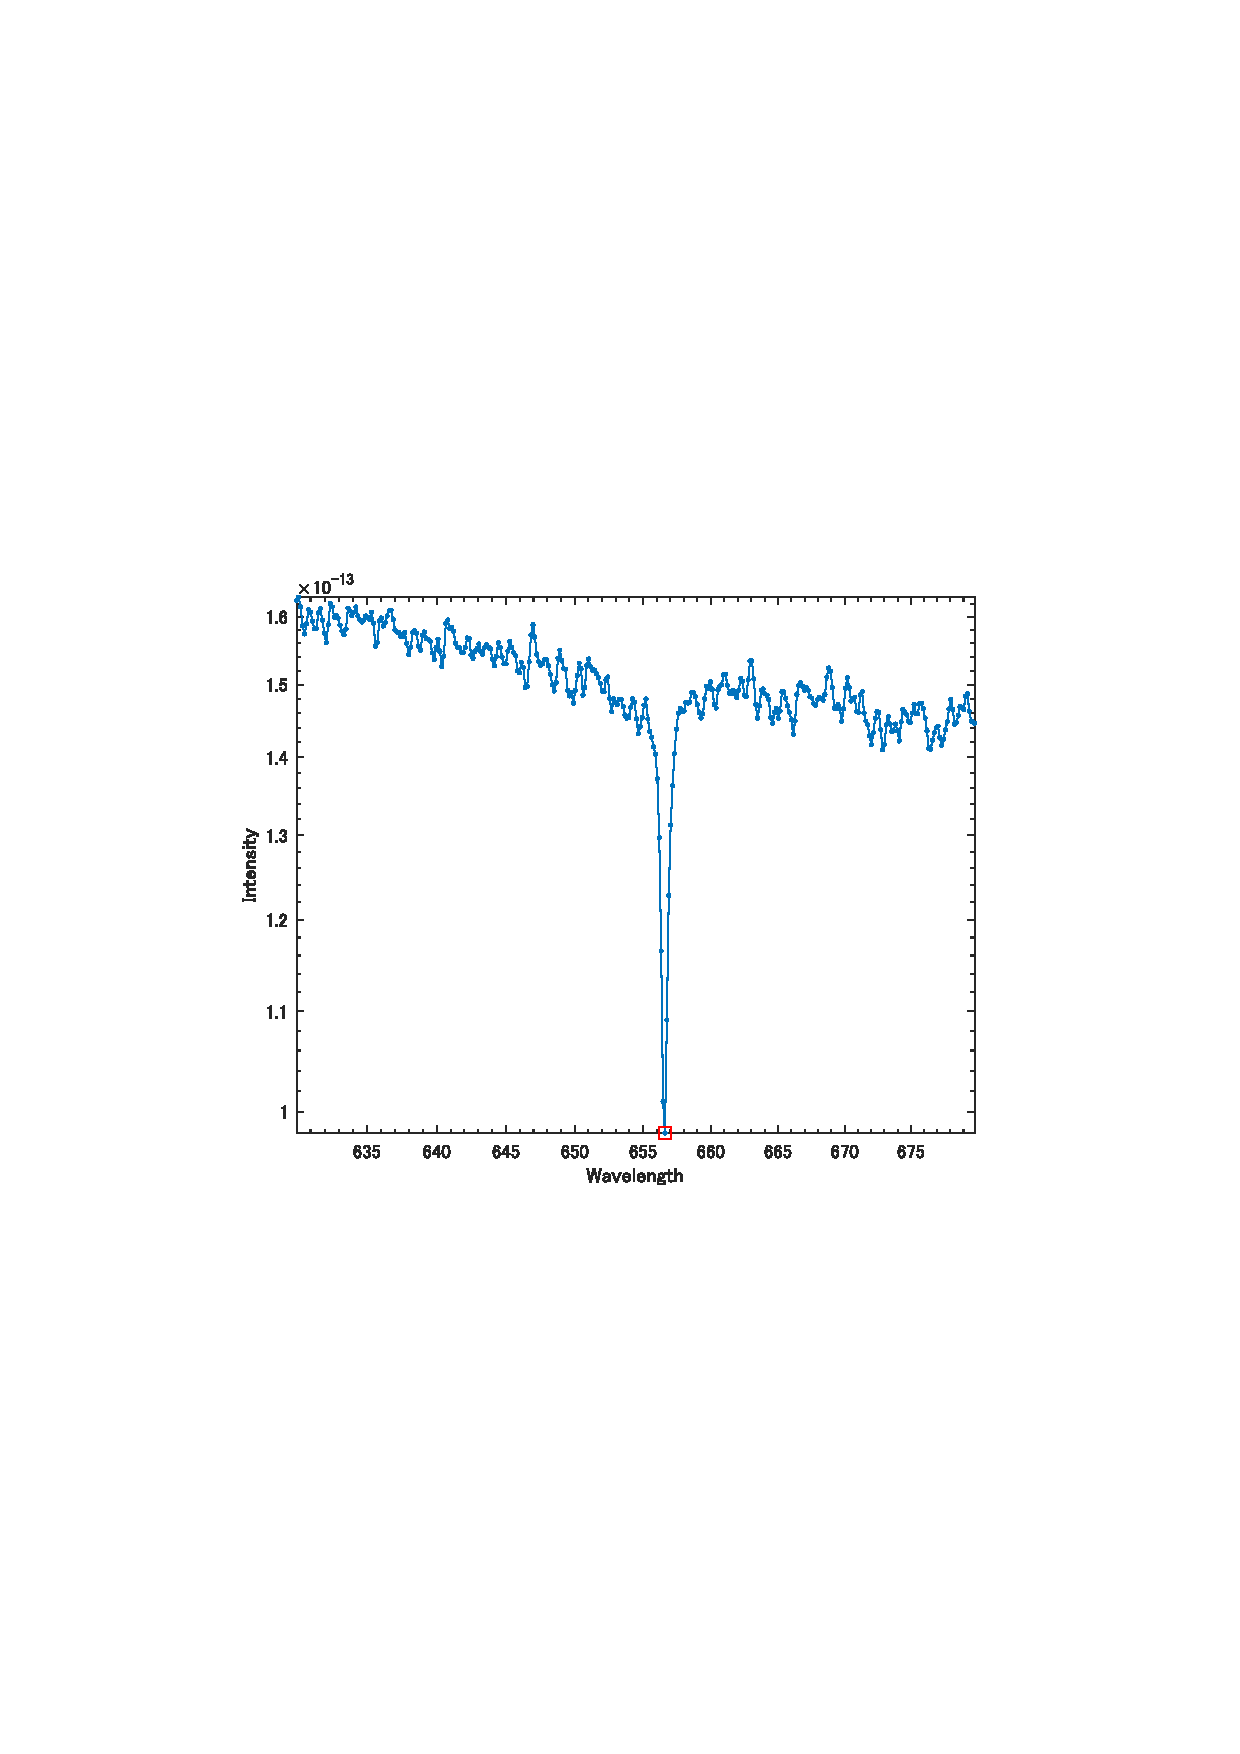
\includegraphics[width=0.5\textwidth]{figure/stellar1.pdf}
        \caption{恒星 HD94028 のスペクトルと水素アルファ線}
        \label{fig:exp3_6_spectra}
    \end{figure}

    ここから,各星の水素アルファ線を求める.行列の各行に対して最小値とそのインデックスを計算する.これは \mintinline{matlab}|min(spectra(:,:))| で求めることができる.また,各星の Ha の波長を \mintinline{matlab}|lambda(idx)|で求め,その値を用いて赤方偏移係数と速度を求める.

    \inputminted[linenos, firstline=11, lastline=15, frame=lines, fontsize=\small]{matlab}{code/Exp3_6_2_Matlab.m}

    この各星で求めた値を1つの図にまとめるプログラムで出力する.全ての星のスペクトルを一つのグラフに目止めて描画し,青方偏移か赤方偏移を視覚的に区別し,どの線がどの星に対応するかを明確にする.各星について速度が 0 以下の場合は青方偏移,0 より大きい場合は赤方偏移と判断するため,if文を用いて条件分岐を行う.また,その条件分岐を各星に対して行うために for 文を用いる.
    \inputminted[linenos, firstline=16, lastline=27, frame=lines, fontsize=\small]{matlab}{code/Exp3_6_2_Matlab.m}

    % svgに変更しよう
    \begin{figure}
        \centering
        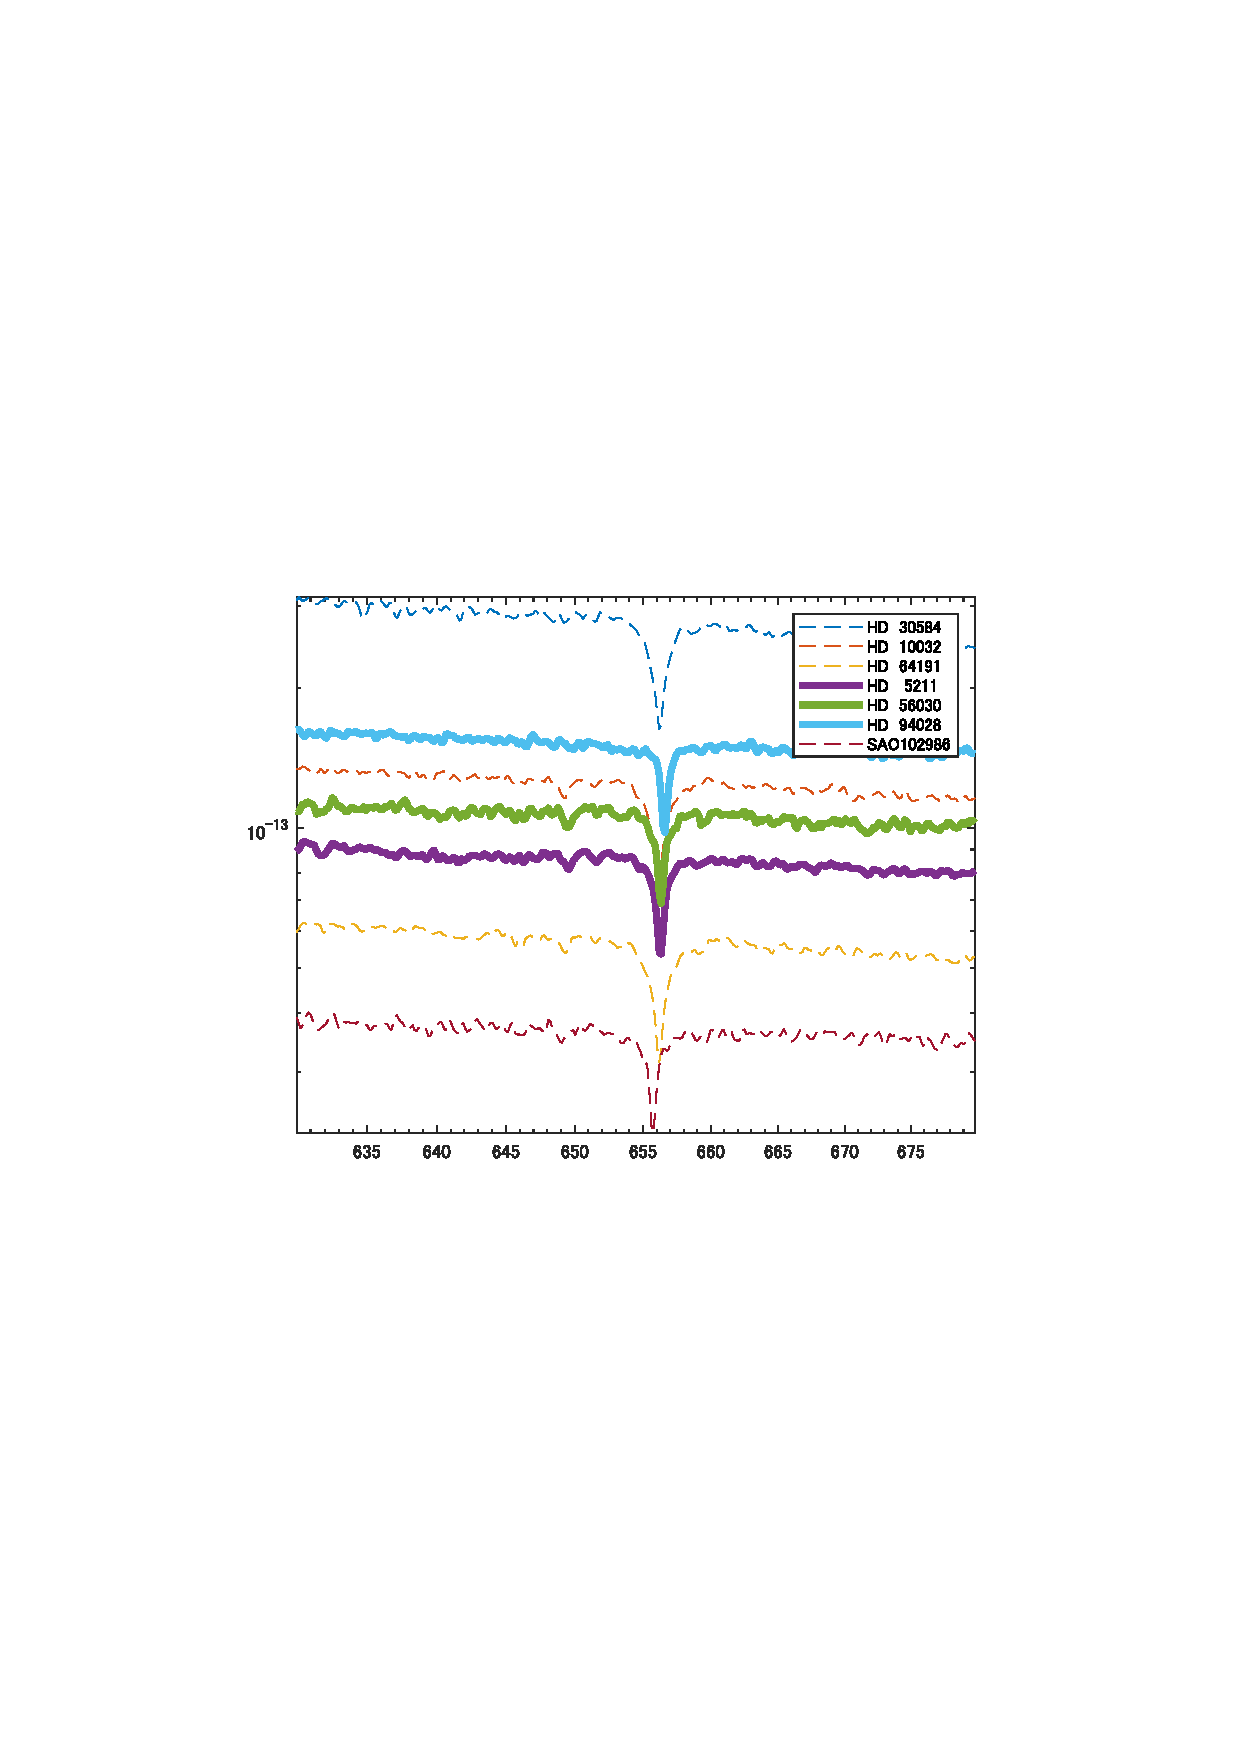
\includegraphics[width=0.5\textwidth]{figure/stellar2.pdf}
        \caption{各星のスペクトルと水素アルファ線}
        \label{fig:exp3_6_spectra2}
    \end{figure}

\section{第七回の方法}
    まず,刺激呈示環境を構築する.まず,背景色を白色とするために \mintinline{matlab}|bgcolor = 255| と設定する.刺激画像の大きさは 640 $\times$ 480 とするので 高さは \mintinline{matlab}|h = 640| とし,幅は \mintinline{matlab}|w = 480| とする.画面左右端と画像端との距離は 220 ピクセルとするため, \mintinline{matlab}|margin = 220| とする.固視点は 画像中央に幅 40,縦 4 及び 幅 4 縦 40 の黒色の十字とする.黒色は 0 で指定することができ,固視点の十字は長方形を二つで組み合わせることで表現できる.ここで長方形は \mintinline{matlab}|[left top right bottom]| でベクトルで定義できる.
    
    \inputminted[linenos, firstline=1, lastline=12, frame=lines, fontsize=\small]{matlab}{code/Exp3_7_Matlab.m}
    \inputminted[linenos, firstline=32, lastline=33, frame=lines, fontsize=\small]{matlab}{code/Exp3_7_Matlab.m}
    \inputminted[linenos, firstline=35, lastline=36, frame=lines, fontsize=\small]{matlab}{code/Exp3_7_Matlab.m}

\end{document}
